\section{Discrete-Time Systems}
\subsection{Discrete-time signal}
\begin{figure}[h!]
    \centering
    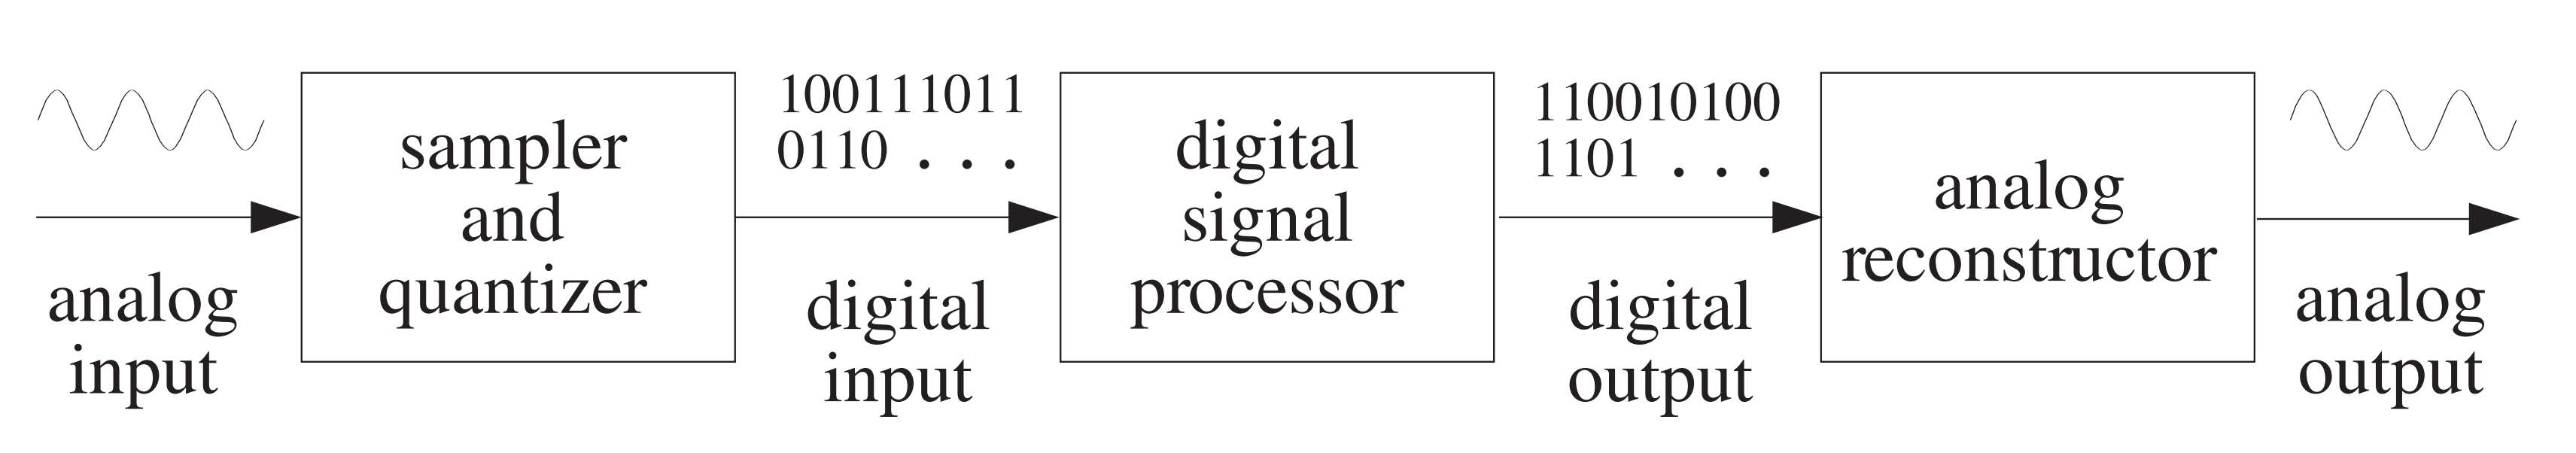
\includegraphics[width=0.7\linewidth]{img/chap3/1.png}
\end{figure}

Unit sample sequence (unit impulse): $\displaystyle \delta(n) \begin{cases}
    1 \quad for\ n=0 \\
    0 \quad for\ n\neq 0
\end{cases} $

Unit step signal: $\displaystyle \delta(n) \begin{cases}
    1 \quad for\ n\geq 0 \\
    0 \quad for\ n< 0
\end{cases} $
\subsection{Input/output rules}
A discrete-time system is a processor that transform an input sequence $x(n)$ into an output sequence $y(n)$.
\begin{figure}[h!]
    \centering
    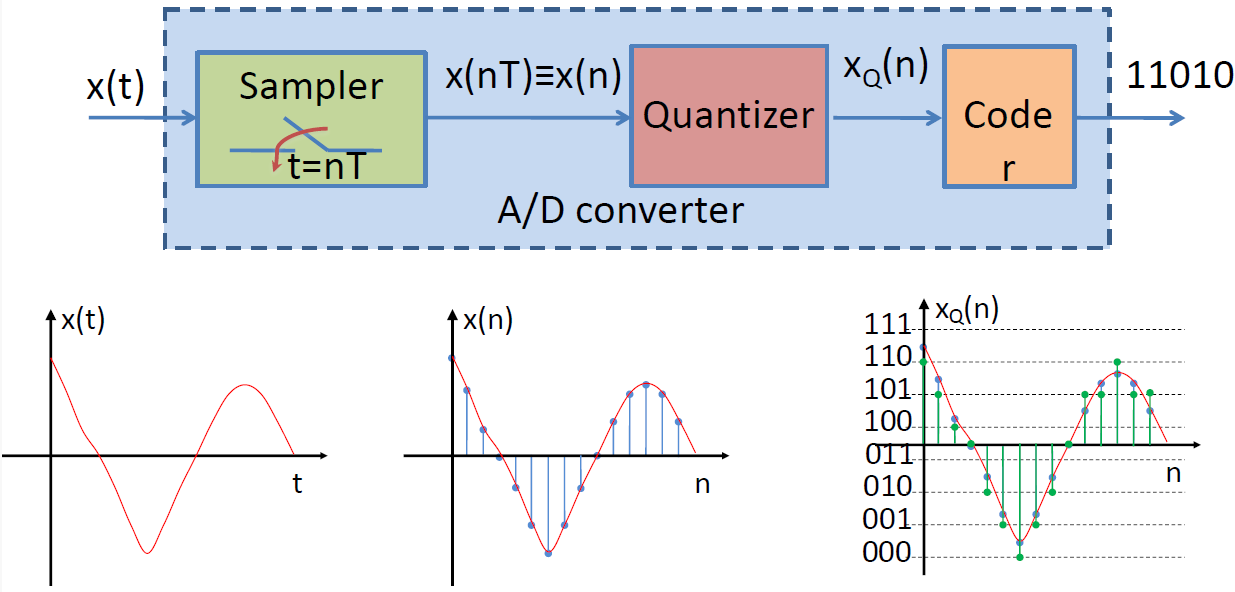
\includegraphics[width=0.4\linewidth]{img/chap3/2.png}
    \caption{Discrete-time system}
\end{figure}

Sample-by-sample processing: $\{x_0,x_1,x_2,...,x_n\} \xrightarrow{H} \{y_0,y_1,y_2,...,y_n\}$ that is, $x_0 \xrightarrow{H}y_0, \ x_1 \xrightarrow{H} y_1,...$ and so on.

Block processing: $x = \begin{bmatrix}
    x_0 \\
    x_1 \\ 
    x_2 \\
    \vdots 
\end{bmatrix} \xrightarrow{H} \begin{bmatrix}
    y_0 \\
    y_1 \\ 
    y_2 \\
    \vdots 
\end{bmatrix}=y$\\
\newpage
\textbf{Basic building blocks of DSP systems}
\begin{figure}[h!]
    \centering
    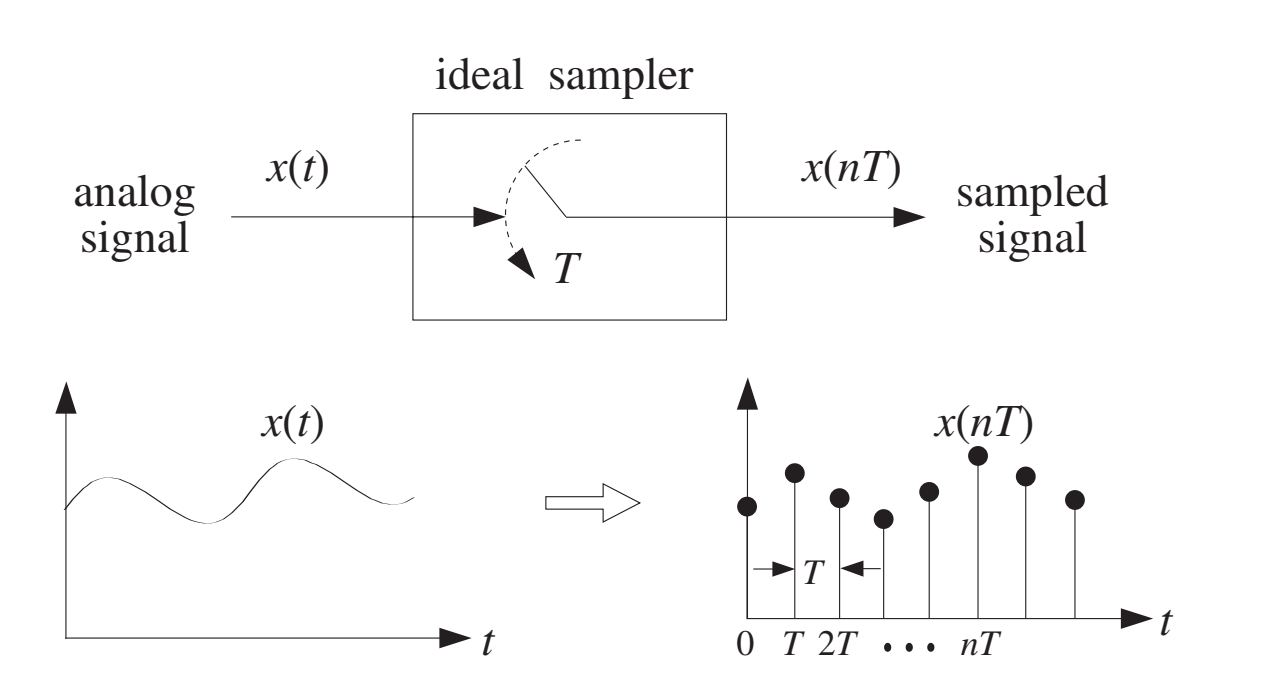
\includegraphics[width=0.5\linewidth]{img/chap3/3.png}
\end{figure}

\subsection{Linearity and time invariance}
A \textbf{linear system} has the property that the output signal due to a linear combination of two input signals can be obtained by forming the same linear combination of the individual outputs.
\begin{figure}[h!]
    \centering
    \includegraphics[width=0.55\linewidth]{img/chap3/4.png}
    \caption{Testing linearity}
\end{figure}

If $x(n)=a_1x_1(n)+a_2x_2(n) \to y(n)=a_1y_1(n)+a_2y_2(n) \ \forall a_1,a_2 \to$ linear system. Otherwise, the system is nonlinear.

A \textbf{time-invariant system} is a system that its input-output characteristics do not change with time.
\begin{figure}[h!]
    \centering
    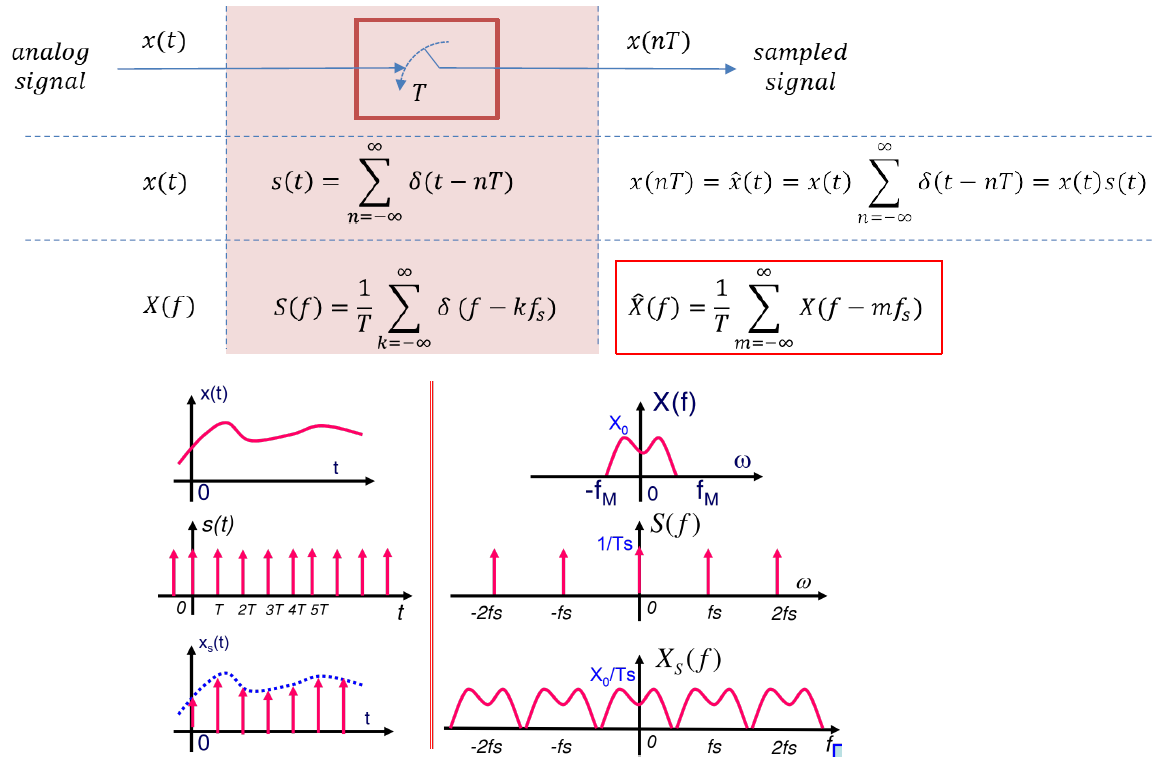
\includegraphics[width=0.4\linewidth]{img/chap3/5.png}
    \caption{Testing time invariance}
\end{figure}

If $y_D(n)=y(n-D) \ \forall D \to$ time-invariant system. Otherwise, the system is time-variant.
\subsection{Impulse response}
\textbf{Linear time-invariant (LTI) systems} are characterized uniquely by their impulse response sequence $h(n)$, which is defined as the response of the systems to a unit impulse $\delta(n)$.
\begin{figure}[h!]
    \centering
    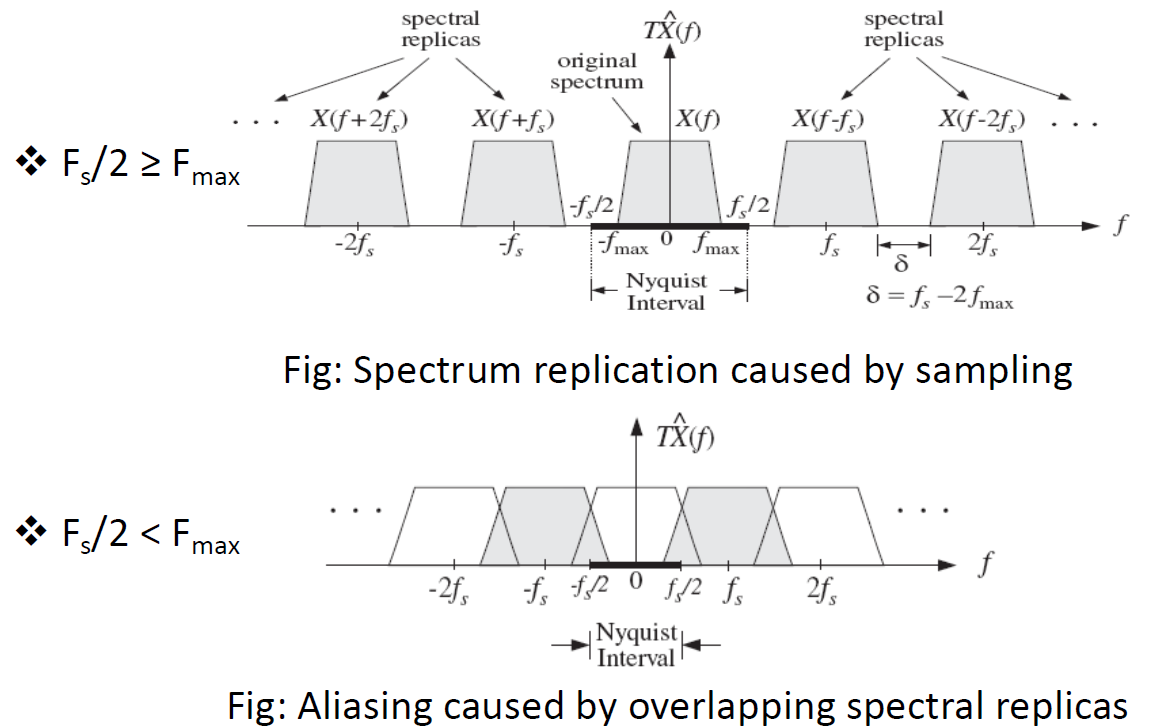
\includegraphics[width=0.5\linewidth]{img/chap3/6.png}
    \caption{Impulse response of an LTI system}
\end{figure}
\begin{figure}[h!]
    \centering
    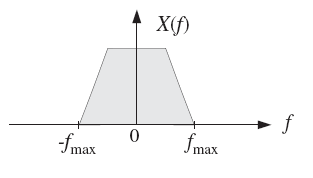
\includegraphics[width=0.5\linewidth]{img/chap3/7.png}
    \caption{Delayed impulse response of an LTI system}
\end{figure}
\subsection{Convolution of LTI systems}
\begin{figure}[h!]
    \centering
    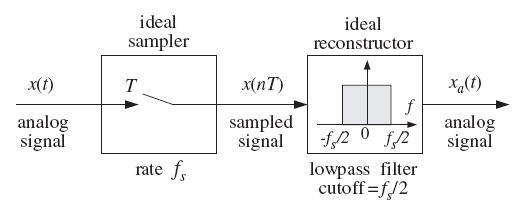
\includegraphics[width=0.5\linewidth]{img/chap3/8.png}
    \caption{Response to linear combination of inputs}
\end{figure}

\textbf{Convolution:}
\begin{equation*}
    y(n) = \sum_{m}x(m)h(n-m)=x(n)*h(n) \quad (\text{LTI form})
\end{equation*}
\begin{equation*}
    y(n) = \sum_{m}h(m)x(n-m)=h(n)*x(n) \quad (\text{direct form})
\end{equation*}
\subsection{FIR versus IIR filters}
A \textbf{finite impulse response (FIR) filter} has impulse response $h(n)$ that extend only over a finite time interval, say $0 \leq n \leq M$.
\begin{figure}[h!]
    \centering
    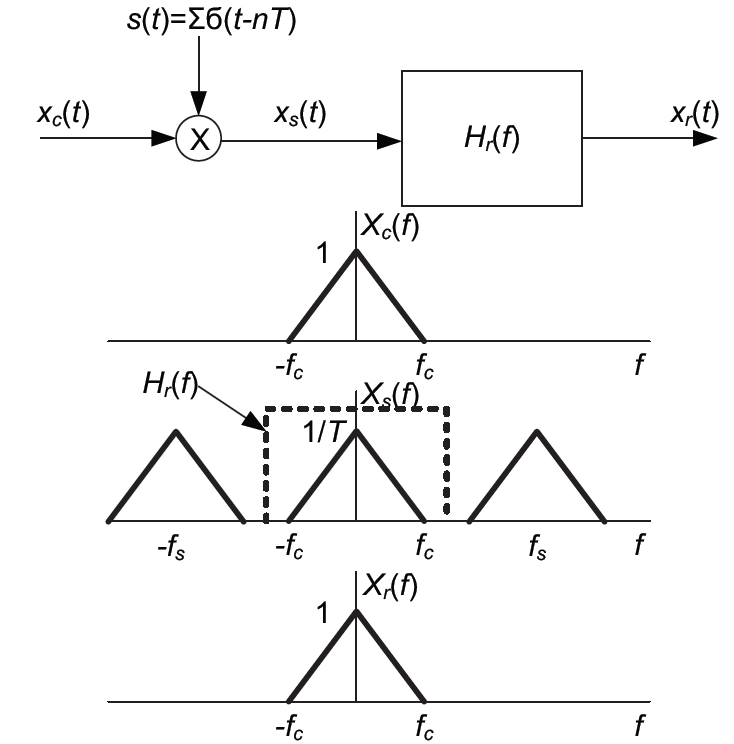
\includegraphics[width=0.3\linewidth]{img/chap3/9.png}
    \caption{FIR impulse response}
\end{figure}
\begin{itemize}
    \item $M$: filter order; $L_h=M+1$: the length of impulse response.
    \item $h=\{h_0,\ h_1,\ ...,\ h_M\}$ is referred by varius name such as filter coefficients, filter weights or filter taps.
    \item FIR filtering equation: $y(n) = \displaystyle\sum_{m=0}^{M}h(m)x(n-m)=h(n)*x(n) $
\end{itemize}
A \textbf{infinite impulse response (IIR) filter} has impulse response $h(n)$ of infinite duration, say $0\leq n \leq\infty$.
\begin{figure}[h!]
    \centering
    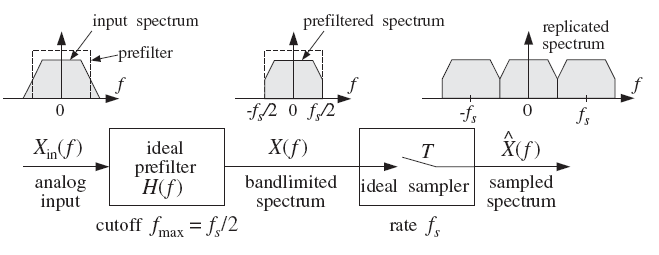
\includegraphics[width=0.3\linewidth]{img/chap3/10.png}
    \caption{IIR impulse response}
\end{figure}

IIR filtering equation: $y(n) = \displaystyle\sum_{m=0}^{M}h(m)x(n-m)=h(n)*x(n) $. The I/O equation of IIR filters are expressed as the recursive differences equation.
\subsection{Causality and Stability}
\begin{figure}[h!]
    \centering
    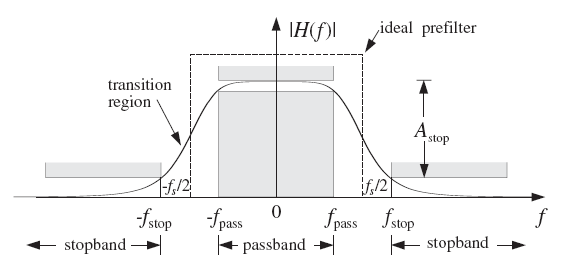
\includegraphics[width=0.5\linewidth]{img/chap3/11.png}
    \caption{Causal, Anticasual and Mixed signals}
\end{figure}

LTI systems can also classified in terms of causality depending on whether $h(n)$ is casual, anticausal or mixed. A system is stable (BIBO) if \textbf{bounded inputs} ($|x(n)| \leq A$) always generate \textbf{bounded outputs} ($|y(n)| \leq B$).

A LTI system is stable $\Leftrightarrow \displaystyle \sum_{n=-\infty}^{\infty} (h(n))<\infty$
\subsection{Static versus Dynamic systems}
Static (memoryless): output at any instant depends at most on the input sample at the same time, but not on past or future samples of the inputs.
\begin{equation*}
    y(n) = \mathcal{J} [x(n),n]
\end{equation*}

Otherwise, the system is dynamic: finite memory, infinite memory.
\subsection{Interconnection of discrete time systems}
\subsection{Energy versus Power signals}
\subsection{Periodic versus Aperiodic signals}